\documentclass[11pt]{article}
\usepackage{graphicx}
\usepackage[a4paper, total={17cm, 27cm}]{geometry}
\title{COMP6245 Lab 3}
\author{James Carlyle}
\date{25 October 2025}
\begin{document}
\maketitle
\section{Task 1: Non-linearly Separable Case}
Train your model on the X-train-nls, y-train-nls dataset. Plot the loss and gradient norm over iterations. You should see both of them converge.
\begin{figure}[h]
    \centering
    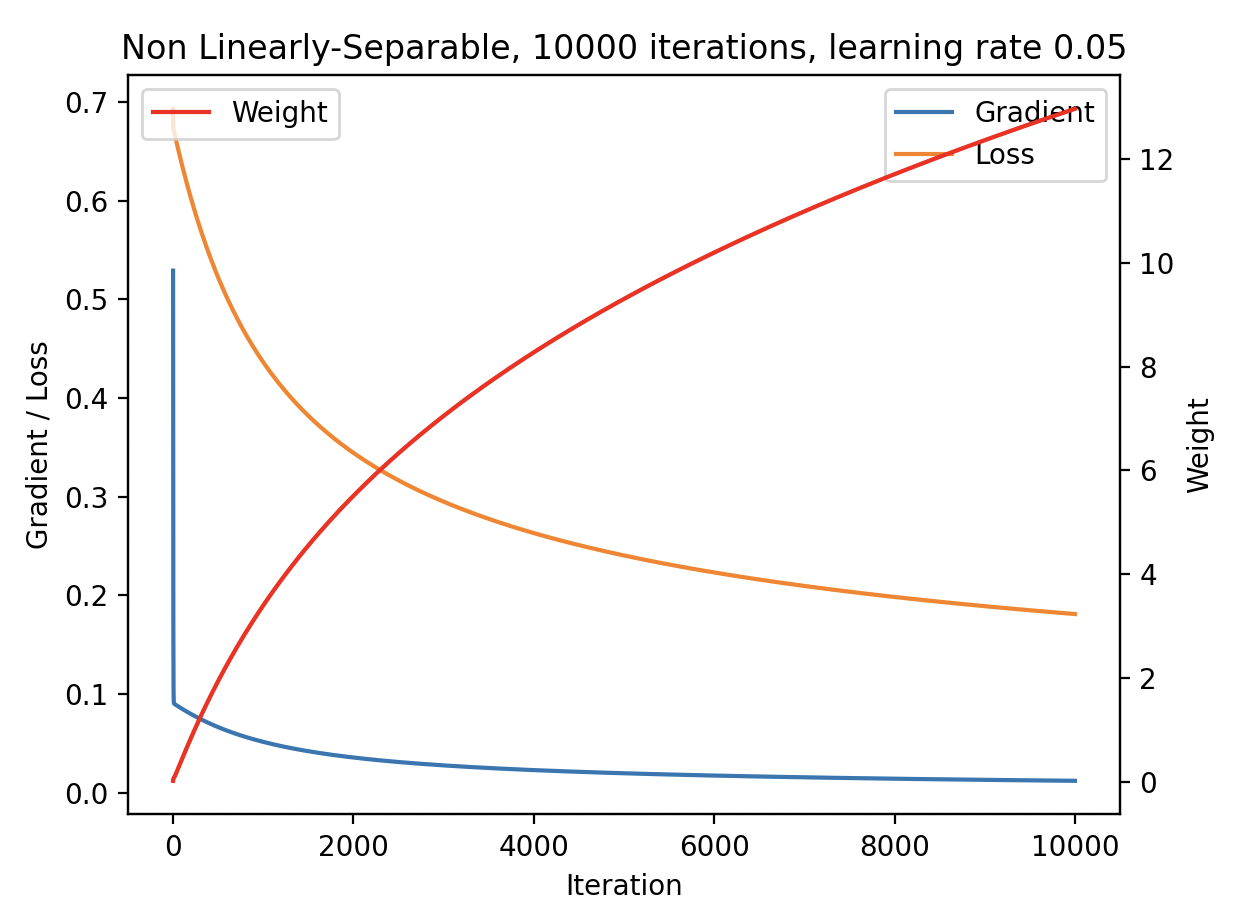
\includegraphics[width=0.5\linewidth]{1.png}
    \caption{Non Linearly separable}
    \label{fig 1}
\end{figure}

Both the gradient and the loss converge, but the weights do not achieve stability after 10,000 iterations.

\section{Task 2: Linearly Separable Case}
Train your model on the X-train-ls and y-train-ls dataset for a large number of iterations (e.g., 5000). Plot the loss and the gradient norm.
\begin{figure}[h]
    \centering
    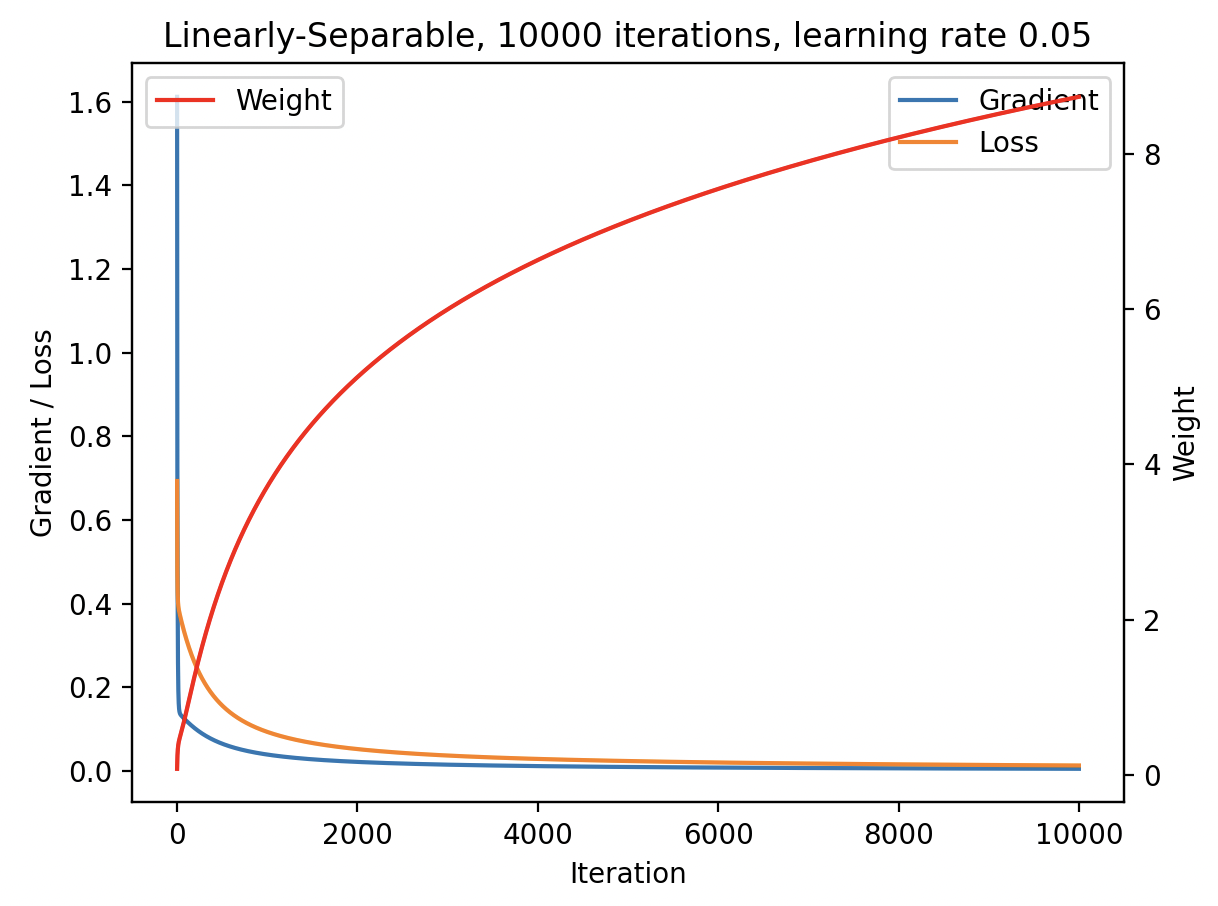
\includegraphics[width=0.5\linewidth]{2.png}
    \caption{Linearly separable}
    \label{fig 2}
\end{figure}

What happens to the loss and gradient norm over time? Explain why this behaviour occurs.
The loss and gradient norm decline over time for both, but the loss decline is much steeper and earlier for the linearly separable case. In both cases, the initial gradient descent is very large, as the initial weights vector was set to zeros. In both cases, the weights do not stabilise but continue to increase even after 10,000 iterations and after the gradient asymptotically approaches a near-zero value.

\section{Task 3: Implement L2 Regularised Logistic Regression}
Re-run the training on the linearly separable training set (X train ls, y train ls) using your new regularised function (e.g., with lambda=0.1).

\begin{figure}[h]
    \centering
    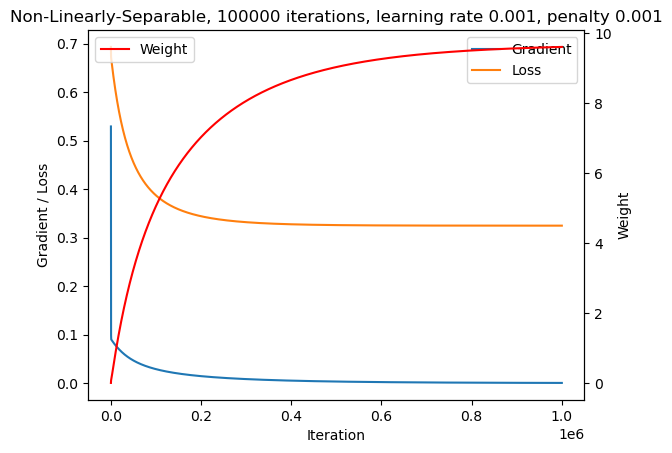
\includegraphics[width=0.5\linewidth]{3.png}
    \caption{Regression with Penalty}
    \label{fig 3}
\end{figure}

Do weights, loss, and gradient norm now converge? Does the magnitude of the final weights compare to the non-regularised version?
Yes, the loss and gradient converge as before, but now the weights also stabilise after about 400 iterations. The magnitude of the weights are significantly smaller than the values seen without regularisation. 

\section{Task 4: Evaluate your Regularized Classifier}
Now, use the regularised model you trained in Step 5 to make predictions on the test set and evaluate its performance.
The model gave the following probabilities output on the test set:
\begin{verbatim}
[0.38641939 0.72001826 0.9493627  0.11256615 0.15745916 0.14492311
 0.36351961 0.82869676 0.03985147 0.26011148 0.31960572 0.06612512
 0.64622582 0.48129585 0.96337717 0.33032437 0.63497602 0.64622582
 0.05032592 0.04376386 0.93059225 0.63497602 0.26962555 0.10316661
 0.37489952 0.23290371 0.12270493 0.73863636 0.1921163  0.90526565]
 \end{verbatim}
 Based on criteria for class selection (probability > 0.5), the following classes are identified:
\begin{verbatim}
[0 1 1 0 0 0 0 1 0 0 0 0 1 0 1 0 1 1 0 0 1 1 0 0 0 0 0 1 0 1]
\end{verbatim}
The binary values represent the two classes.

\begin{verbatim}
- - - Classification Report - - -
              precision    recall  f1-score   support

           0       0.89      1.00      0.94        17
           1       1.00      0.85      0.92        13

    accuracy                           0.93        30
   macro avg       0.95      0.92      0.93        30
weighted avg       0.94      0.93      0.93        30    
\end{verbatim}

\begin{figure}[h]
    \centering
    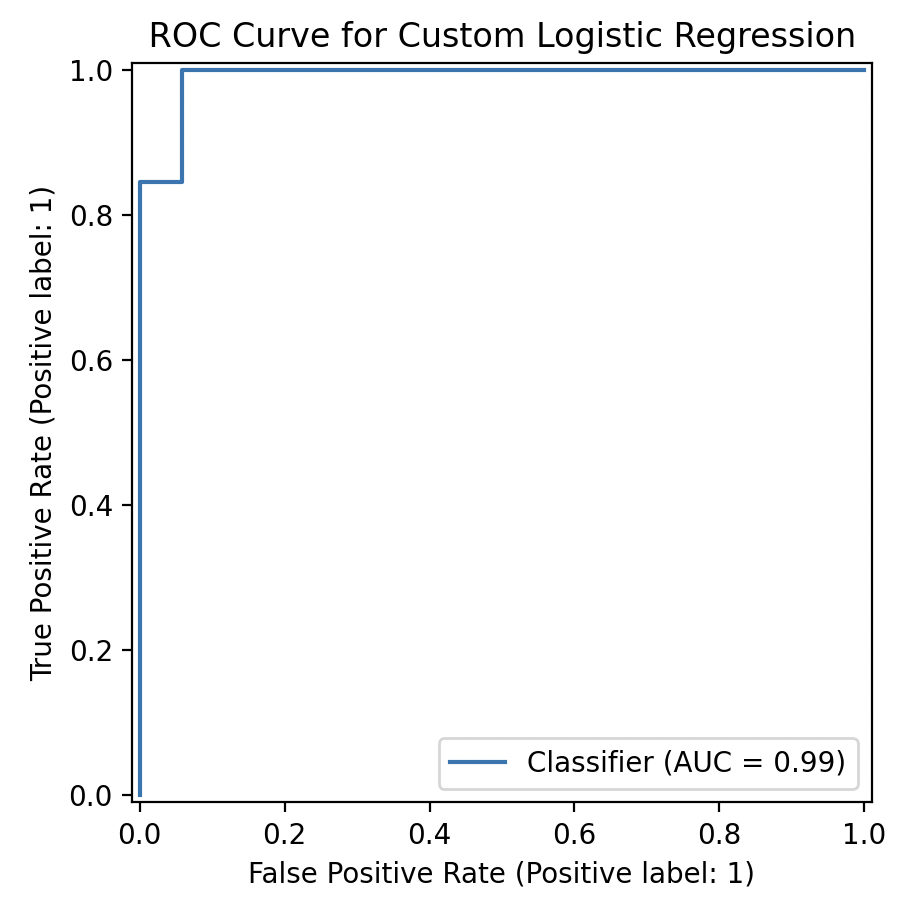
\includegraphics[width=0.5\linewidth]{4.png}
    \caption{ROC Curve for custom logistic regression}
    \label{fig 4}
\end{figure}

\begin{verbatim}
- - - Confusion Matrix - - -
[[17  0]
 [ 2 11]]

AUC Score : 0.9910
\end{verbatim}
\section{Part 2: Naive Bayes}
\section{Task 1: Intuition Building - Spam Classification by Hand}
\subsection{1. Calculate Class Priors: Calculate the prior probabilities, P(Spam) and P(Ham).}
\begin{verbatim}
p-spam 0.4
p-not-spam 0.6
\end{verbatim}

\subsection{2. Calculate Word Likelihoods: Calculate P(word|Class) for ”free” and ”call” using the add-one smoothing formula:}
\begin{verbatim}
Word Free spam score is 0.0952  = P(free|spam)
Word Free not spam score is 0.0370 = P(free|not spam)
Word Call spam score is 0.0952 = P(call|spam)
Word Call not spam score is 0.0741 = P(call|not spam)
\end{verbatim}

\subsection{3. Calculate Posterior Probabilities: Calculate scores proportional to the posterior for each class.}
To complete the sentence the remaining word likelihoods are: 
\begin{verbatim}
P(for|spam) = (0 + 1) / (7 + 14) = 0.0476
P(for|not spam) = (0 + 1) / (13 + 14) = 0.0370
P(you|spam) = (0 + 1) / (7 + 14) = 0.0476
P(you|not spam) = (2 + 1) / (13 + 14) = 0.1111
\end{verbatim}

Multiplying terms, 
\begin{verbatim}
P("free call for you"|spam) = 0.0000205
P("free call for you"|not spam) = 0.0000112
\end{verbatim}

Bayes Theorem gives
\begin{equation}
    P(class|words) = P(words|class)*P(class) / P(words)
\end{equation}

\begin{verbatim}
For class Spam, 
P(spam|"free call for you") = 0.0000205 * 0.4 / P(words) = 0.00000821
For class Not spam, 
P(not spam|"free call for you") = 0.0000112 * 0.6 / P(words) = 0.00000676
\end{verbatim}

The divisor P(words) can be ignored as it is the same term for both probabilities.

\subsection{4. Classify the Message: Based on your scores, which class is more likely?}
We determine that the message "free call for you" is more probably spam.

\section{Task 2: Application - Real-World Text Classification}
\subsection{Step 4: Hands-On Analysis - Looking Inside the Model}
The following results were generated:
\begin{verbatim}
                     precision    recall  f1-score   support

         sci.space       0.97      0.99      0.98       394
talk.religion.misc       0.99      0.96      0.97       251

          accuracy                           0.98       645
         macro avg       0.98      0.98      0.98       645
      weighted avg       0.98      0.98      0.98       645
\end{verbatim}

\begin{verbatim}
Model's Prediction : 'talk.religion.misc '
Score(sci.space) = -698.6741
Score(talk.religion.misc) = -617.9126

Prediction: 'talk.religion.misc'
Match: True
\end{verbatim}

This confirms that the predicted topic for the dataset is the same as the manually generated prediction.
\end{document}